\mySection{10.2 The Multinomial Distribution}
%-------------- start slide -------------------------------%{{{ 10.8
\begin{frame}
	% {\S\: 10.2 The Multinomial Distribution}
	
\includegraphics[scale=0.5]{MM-neg.jpeg}
\begin{enumerate}
\item[Def.] Suppose one does an experiment of extracting $n$ balls of $t$ different colors from a jar,
	replacing the extracted ball after each draw.
	Balls from the same color are equivalent.
	Denote the variable which is the number of extracted balls of color $i$ ($i = 1, ..., t$) as $X_i$,
	and denote as $p_i$ the probability that a given extraction will be in color $i$.
	The probability distribution function of the vector $(X_1,\cdots,X_t)$ is called
	the \textcolor{yellow}{multinomial distribution}, which is equal to
	\begin{align*}
		p_{X_1,\cdots,X_t}(k_1,\cdots,k_t)
		&= \bbP\left( X_1=k_1,\cdots,X_t=k_t \right)\\
		&= {n\choose k_1,\cdots,k_t} p_1^{k_1}\cdots p_t^{k_t}
	\end{align*}
	where $k_i\in\{0,1,\cdots, n\}$, $1\le i\le t$, $\sum_{i=1}^t k_i=n$, and $p_1+\cdots+p_t=1$.
\end{enumerate}
\end{frame}
%-------------- end slide -------------------------------%}}}
%-------------- start slide -------------------------------%{{{ 10.9
\begin{frame}
	% {Properties of multinomial distribution}
	\begin{enumerate}
		\item[Thm] Suppose $(X_1,\cdots, X_t)$ follows the multinomial distribution with parameters $n$ and $(p_1,\cdots,p_t)$ with $p_i\ge 0$ and $\sum_{i}p_i=1$. Then\\[1em]
		\item $X_i\sim$Binomail($n,p_i$) and hence\\[2em]
		\item[] $\E[X_i] = n p_i$
		\item[] $\Var(X_i) = n p_i(1-p_i)$
		\vfill
		\item $\text{Cov}(X_i,X_j) = -np_ip_j$, $i\ne j$. \hfill (negative correlated)
		\vfill
		\item $M_{X_1,\cdots,X_t}(s_1,\cdots,s_t) = \left(p_1e^{s_1} + \cdots + p_t e^{s_t} \right)^n$.
	\end{enumerate}
\end{frame}
%-------------- end slide -------------------------------%}}}
%-------------- start slide -------------------------------%{{{ 10.10
\begin{frame}[fragile]

	\begin{enumerate}
		\item[Proof]
		\item[(3)]
\begin{align*}
	M_{X_1,\cdots,X_t}(s_1,\cdots,s_t) & = \E \left[e^{X_1 s_1+\cdots+X_t s_t} \right ]                                                                                        \\
                                     & = \mathop{\sum_{k_1,\cdots,k_t=0}^n}_{k_1+\cdots+k_t=n} {n\choose k_1,\cdots,k_t} p_1^{k_1}\cdots p_t^{k_t}e^{k_1 s_1+\cdots+k_t s_t} \\
                                     & = \mathop{\sum_{k_1,\cdots,k_t=0}^n}_{k_1+\cdots+k_t=n} {n\choose k_1,\cdots,k_t} (p_1e^{s_1})^{k_1}\cdots (p_te^{s_t})^{k_t}         \\
                                     & = \left(p_1e^{s_1}+\cdots+p_te^{s_t} \right)^n
\end{align*}
\vfill
\item[(1)] To find $M_{X_i}(s_i)$, we simply set $s_j\equiv 0$ for $j\ne i$. Hence
	\[
		M_{X_i}(s_i) = \big(\underbrace{p_1+\cdots+p_{i-1}+p_{i+1}+\cdots+p_t}_{=1-p_i}+p_ie^{s_i} \big)^n
		\:\Longrightarrow\:
		\text{$X_i\sim$ Binomial$(n,p_i)$}
	\]
	\end{enumerate}
\end{frame}
%-------------- end slide -------------------------------%}}}
%-------------- start slide -------------------------------%{{{ 10.11
\begin{frame}[fragile]

	\begin{enumerate}
		\item[(2)] Set $M:=M_{X_1,\cdots,X_t}(s_1,\cdots,s_t)$. Then for $i\ne j$,
		\item[]
			\begin{align*}
				\frac{\partial M}{\partial s_i} =n \left(p_1e^{s_1}+\cdots+p_te^{s_t} \right)^{n-1} p_i e^{s_i}
			\end{align*}
		\item[]
			\begin{align*}
				\frac{\partial^2 M}{\partial s_i\partial s_j} =n(n-1) \left(p_1e^{s_1}+\cdots+p_te^{s_t} \right)^{n-2} p_i e^{s_i}p_j e^{s_j}
			\end{align*}
		\item[]
			\[
			\Downarrow
			\]
			\[
		\E[X_iX_j] = \frac{\partial^2 M}{\partial s_i\partial s_j}\bigg|_{s_1=\cdots=s_t=0}= n(n-1)(p_1+\cdots+p_t)^{n-2}p_ip_j			=n(n-1)p_ip_j\]
	\item[]
		\[\Downarrow\]
		\begin{align*}
			\Cov(X_i,X_j)
		&= \E[X_iX_j] - \E[X_i]\E[X_j]
	      \\&= n(n-1)p_ip_j - np_i\times np_j \\
		&= - np_ip_j
		\end{align*}
		\myEnd
	\end{enumerate}
\end{frame}
%-------------- end slide -------------------------------%}}}
%-------------- start slide -------------------------------%{{{ 10.12
\begin{frame}

From a continuous pdf to a multinomial distribution:
\vfill
\begin{enumerate}
	\item[E.g.] Let $Y_i$ be a random sample of size $n$ from $f_Y(y)=6y(1-y)$, $y\in[0,1]$.
		Define
		\[
		X_i =
		\begin{cases}
			1 & Y_i \in [0,0.25)\\
			2 & Y_i \in [0.25,0.5)\\
			3 & Y_i \in [0.5,0.75)\\
			4 & Y_i \in [0.75,1)
		\end{cases}
		\]
		Find the distribution of $(X_1,\cdots,X_n)$.
		\vfill
	\item[Sol.] $(X_1,X_2,X_3,X_4)$ follows multinomial distribution with parameters $(p_1,p_2,p_3,p_4)$ where
		\begin{align*}
			p_1 = \int_0^{\frac{1}{4}}6y(1-y)dy = \cdots = \frac{5}{32},
		\end{align*}
\end{enumerate}
\end{frame}
%-------------- end slide -------------------------------%}}}
%-------------- start slide -------------------------------%{{{ 10.13
\begin{frame}
\centering
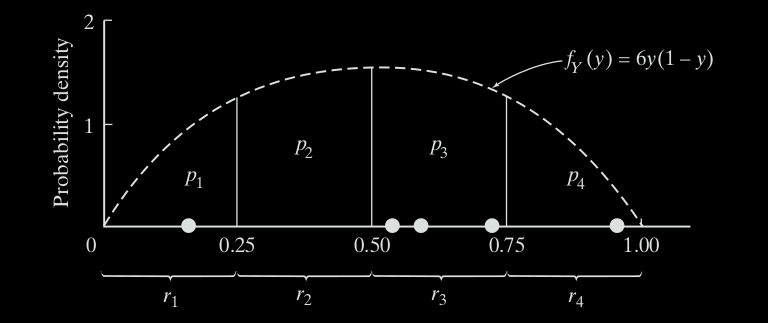
\includegraphics[scale=0.35]{Figure_10-2-2-neg.png}
\vfill
\begin{enumerate}
	\item[] and by symmetry,
		\begin{align*}
			 p_4=p_1=\frac{5}{32}\quad\text{and}\quad
			 p_2=p_3 = \frac{1}{2}\left(1-p_1-p_4\right) = \frac{11}{32}.
		\end{align*}
		\myEnd
		\bigskip
	\item[Remark] In this way, we transform the outcomes, any values between $[0,1]$, into \textcolor{yellow!80!black}{\bf categorical data}.
This chapter is about
\item[]
		\begin{center}
		\bf Analysis of Categorical Data
		\end{center}
\end{enumerate}
\end{frame}
%-------------- end slide -------------------------------%}}}
